\documentclass[aspectratio=169,usenames,dvipsnames]{beamer}
\usepackage{preamble}

\title{Coding for Humanities}
\author{Andreas van Cranenburgh}
\date{Week 6: Exploratory data analysis with Pandas}

\begin{document}
\maketitle


\begin{frame}{Last week}
    Improving code

    \vspace{1em}
    Sentiment analysis

    \vspace{1em}
    Keyword analysis
\end{frame}

\begin{frame}{Program for today}
\tableofcontents
\end{frame}


\section{Midterm feedback}

\begin{frame}{Midterm feedback}
    \begin{itemize}
        \item Most of your code was pretty good!
        \item We'll review some things to pay attention to.
    \end{itemize}
\end{frame}

\begin{frame}{Always report requested results!}
    Read the questions carefully. \\
    When results are requested, include them!

    \vspace{1em}
    \begin{itemize}
        \item Suppose that we call function \textcolor{blue}{\texttt{a}}
            as follows: [...]\\
            What values will be printed to the screen?
        \item Use [your function] to print all tweets addressed to @FLOTUS.
        \item Count the \#hashtags and \@usernames in Trump's tweets, and
            report the top 10 for both.
    \end{itemize}
\end{frame}


\begin{frame}[fragile]{Functions: return vs print}
Write a function first\_letters(filename) that reads a poem in a text file
\structure{and returns a string of first letters} of all of its lines.
\vspace{1em}
\begin{columns}
\column{0.5\textwidth}
Don't print inside the function:
\begin{lstlisting}[style=smaller]
def first_letters(text):
    punctuation = '...'
    for char in punctuation:
        text = text.replace(char, '')
    for line in text.splitlines():
        print(line[0])
\end{lstlisting}
\pause\column{0.5\textwidth}
Collect and \structure{return} the result: 
\begin{lstlisting}[style=smaller]
def first_letters(text):
    punctuation = '...'
    for char in punctuation:
        text = text.replace(char, '')
    result = ''
    for line in text.splitlines():
        result += line[0]
    return result
\end{lstlisting}
\end{columns}
\end{frame}

\begin{frame}[fragile]{Functions: making re-usable functions}
\begin{lstlisting}[style=smaller]
prefix = '@'

def filter_ats(tokens, prefix):
    newlist = [k for k in tokens if prefix in k]
    return newlist

usernames = filter_ats(tokens, prefix)

prefix2 = '#'

def filter_hashtags(tokens, prefix2):
    newlist = [k for k in tokens if prefix2 in k]
    return newlist

hashtags = filter_hashtags(tokens, prefix2)
\end{lstlisting}

(BTW: great use of list comprehensions)
\end{frame}

\begin{frame}[fragile]{Functions: making re-usable functions}
One re-usable function: 
\begin{lstlisting}[style=smaller]
def filter_tokens(tokens, prefix):
    newlist = [token for token in tokens
            if token[0] == prefix]
    return newlist

usernames = filter_tokens(tokens, '@')
hashtags = filter_tokens(tokens, '#')
\end{lstlisting}

Lesson:
    \begin{itemize}
        \item Don't Repeat Yourself (DRY)
        \item one function can do multiple jobs,
            based on its arguments
    \end{itemize}
\end{frame}

\begin{frame}[fragile]{Function scope}
    \begin{definition}
        The \structure{scope} of a variable determines which parts of your code \\
            can access a variable.
    \end{definition}
    \begin{description}
        \item[global scope] variables created outside a function.
            \begin{itemize}
                \item Everyone can see them.
                \item Available all the time.
            \end{itemize}
        \item[local scope] arguments and variables created in a function.
            \begin{itemize}
                \item Other code cannot see them.
                \item Created and destroyed for each function call.
            \end{itemize}
    \end{description}
\end{frame}


\begin{frame}[fragile]{What if there are more than 2 punctuation marks?}
    \begin{columns}[T]
\column{0.6\textwidth}
Skipping only the first punctuation mark is not enough!
\begin{lstlisting}[style=plain]
- ``Shall I compare thee ...''
- ``Please don't!'' she replied
\end{lstlisting} % SPAM
\pause\column{0.4\textwidth}
Solution: remove all punctuation
\begin{lstlisting}[style=plain]
Shall I compare thee
Please dont
\end{lstlisting}
\end{columns}
Lesson:
    \begin{itemize}
        \item Don't just test your code \\
            on the particular given examples.
        \item Tests are typically not exhaustive.
        \item Reflect whether you really solved the problem.
    \end{itemize}
\end{frame}

\begin{frame}[fragile]{For loops: premature return}
\begin{columns}
\column{0.5\textwidth}
Pay attention to what is part of a for loop!
\begin{lstlisting}
result = []
for line in text.splitlines():
    result += line[0]
    return result
\end{lstlisting}
Why does this not work?
\pause\column{0.5\textwidth}
\texttt{return} immediately aborts the function!
\begin{lstlisting}
result = []
for line in text.splitlines():
    result += line[0]
return result
\end{lstlisting}
\end{columns}
\end{frame}

\begin{frame}[fragile]{For loops: inefficiency}
\begin{columns}[T]
\column{0.5\textwidth}
Pay attention to what is part of a for loop!
\begin{lstlisting}
chars = []
for line in text.splitlines():
    chars.append(line[0])
    result = ''.join(chars)
return result
\end{lstlisting}
\pause
This repeats the join at every iteration, completely unnecessary!
\column{0.5\textwidth}
Solution: Take the join out of the for loop:
\begin{lstlisting}
chars = []
for line in text.splitlines():
    chars.append(line[0])
result = ''.join(chars)
return result
\end{lstlisting}
\end{columns}
\end{frame}

\begin{frame}[fragile]{Only concatenate same types!}
\begin{columns}[T]
\column{0.5\textwidth}
Don't do this:
\begin{lstlisting}
result = []
for line in text.splitlines():
    result += line[0]
\end{lstlisting}
Why not? \pause
Type mismatch:
    \begin{itemize}
        \item \texttt{result} is a list
        \item \texttt{line[0]} is a string \\
            (of one character).
    \end{itemize}
\column{0.5\textwidth}
Better:
\begin{lstlisting}
result = ''
for line in text.splitlines():
    result += line[0]
\end{lstlisting}
Best:
\begin{lstlisting}
return ''.join(line[0] for line
        in text.splitlines())
\end{lstlisting}
\end{columns}
\end{frame}


\begin{frame}{Summary}
    Most of your code was pretty good!
    
    \vspace{1em}
    Pay attention to:
    \begin{itemize}
        \item functions
        \item indentation
        \item types
    \end{itemize}
\end{frame}





\section{Exploratory Data Analysis}
\frame{\tableofcontents[currentsubsection]}

\begin{frame}{Data Science}
\begin{reference}
    \url{http://www.datasciencecourse.org/notes/intro/}
\end{reference}
    \begin{definition}
    \structure{Data science} is the application of
    computational and statistical techniques to
    address or gain % [managerial or scientific]
    insight into some problem in the real world. \\
    --- Zico Kolter, Machine Learning Prof, CMU
    \end{definition}
\end{frame}


\begin{frame}
    \centering
    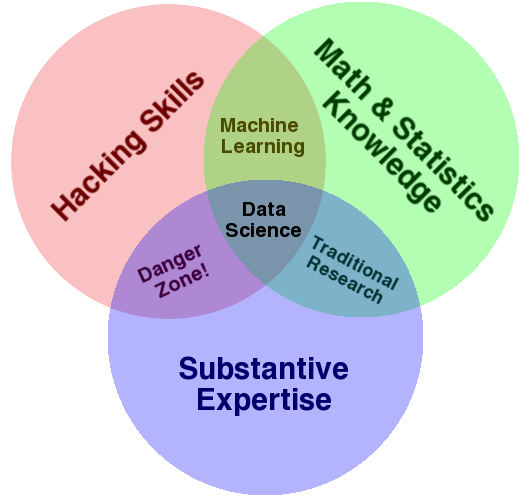
\includegraphics[height=0.8\textheight]{fig/venn}

    Drew Conway

    CEO, Alluvium (analytics company)
\end{frame}


\begin{frame}{The Data Lifecycle}
    \begin{enumerate}
        \item Data collection
        \item Data processing
        \item \structure{Exploratory data analysis \& visualization}
        \item ``Confirmatory data analysis'' \\
            Hypothesis testing, Machine Learning
        \item Insight \& Policy Decision
    \end{enumerate}

    \vspace{1em}
    This course focuses on step 3
\end{frame}

\begin{frame}{Data Collection, Processing}
In practice, this often takes the most time (up to 80\%!)

\begin{itemize}
    \item Acquiring data
        \begin{itemize}
            \item Scrape from web, PDFs
            \item Database dump
            \item etc.
        \end{itemize}
    \item Messy data: encoding issues, date formats, order of first/last names, etc.
    \item Missing data
    \item Converting data
        \begin{description}
            \item[Tidy format] one observation per row, \\
                    each variable is a column
        \end{description}
\end{itemize}
\end{frame}



\begin{frame}{Types of variables}
    \begin{description}
        \item[Continuous] numerical variables\\
            age, length, etc.
        \item[Categorical] predefined set of values\\
            yes/no, True/False, red/blue/green, etc.
        \item[Text] open-ended, unstructured \\
            comments, tweets, etc.
    \end{description}
\end{frame}

\begin{frame}{Descriptive statistics}
%Part of \structure{descriptive statistics}, used to summarize data:
%\begin{itemize}
%    \item Convey lots of information with extreme simplicity
%\end{itemize}
\structure{Descriptive statistics} contrasts with inferential statistics
    (hypothesis testing)

\vspace{1em}
Descriptive statistics for one variable:
\begin{itemize}
    \item Distribution: bar plot, histogram
    \item Measures of location: mean, median
    \item Measure of dispersion: range, standard deviation
\end{itemize}

\pause
Interaction of two variables (next week):
\begin{itemize}
    \item Contingency table, multi-panel plot, scatter plot
    \item Understanding, measuring correlation
\end{itemize}
\end{frame}

\subsection{Exploring one variable}
\frame{\tableofcontents[currentsubsection]}

\begin{frame}{Plotting a distribution: categorical}
Collected favorite color of 100 people:

[black, green, green, blue, red, \dots ]

\vspace{1em}
How do we visualize this?

\pause\vspace{1em}
\begin{columns}
\column{0.46\textwidth}
A bar plot:

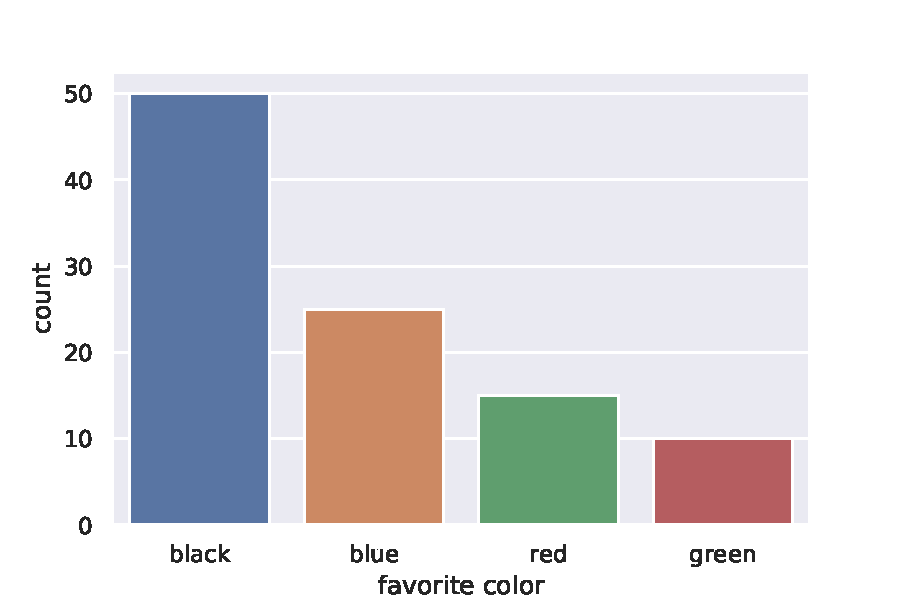
\includegraphics[height=0.55\textheight]{fig/barplot}

\column{0.46\textwidth}
Don't use a pie chart: \url{https://www.businessinsider.com/pie-charts-are-the-worst-2013-6}
\end{columns}
\end{frame}


\begin{frame}{Plotting a distribution: continuous}
Collected height of 100 people:

[1.85, 1.66, 1.77, 1.68, \dots]

\vspace{1em}
How do we visualize this?

\pause
\begin{columns}[T]
\column{0.5\textwidth}
A histogram:

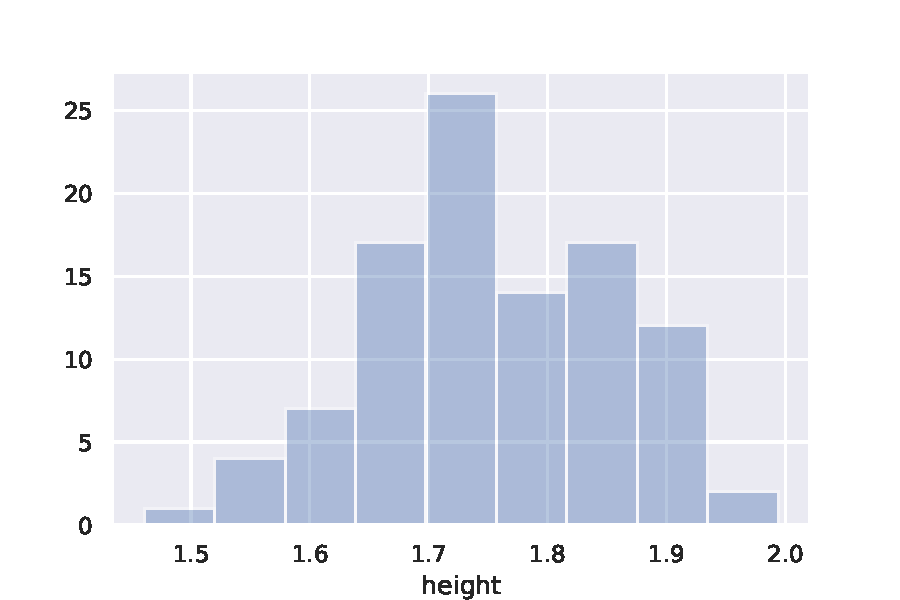
\includegraphics[height=0.55\textheight]{fig/histogram}
\column{0.5\textwidth}
\begin{itemize}
    \item Data points are put in bins \\
        (e.g., 1.70-- 1.76)
        \vspace{1em}

    \item Y-axis: number of datapoints in each bin
        (e.g., 26 for 1.70--1.76)
        \vspace{1em}

    \item Number \& width of bins
        chosen automatically or manually
\end{itemize}
\end{columns}
\end{frame}



\begin{frame}{Average house price in each US state}
\begin{columns}
\column{0.5\textwidth}
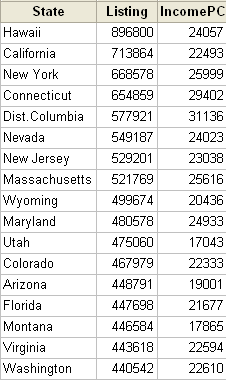
\includegraphics[height=0.8\textheight]{fig/housepricesincome}
\column{0.5\textwidth}
What is the average price \\
across the whole US?

\pause\vspace{1em}
price = (hawaii + california \\
    + ... ) / 50 = \$ 369,687

\vspace{1em}
Is this a fair summary?
\end{columns}
\end{frame}

\begin{frame}{Averaging averages?}
\structure{But}:

Hawaii's average listing = \$896,800\\
Hawaii's population = 1,275,194\\
Illinois' average listing = \$377,683\\
Illinois' population = 12,763,371

\vspace{1em}
Each state gets a weight of 1/50.\\
Hawaii would have too much influence.

\pause
\structure{Better}:
\begin{block}{Weighted average}
price = (weight$_1 \times $value$_1$ + weight$_2 \times $value$_2$ + \dots)

    where weight is population$_{\textsf{state}}$ / population$_{\textsf{total}}$
\end{block}

\vspace{1em}
New average is \$409,234 compared to \$369,687 without weights, \\
an error of 11\%
\end{frame}


\begin{frame}{Mean and median}
    `Average' can mean different things:
    \begin{description}
        \item[(Arithmetic) Mean] sum of values, divided by number of values \\
                Mean[1,2,4,6,8,9,17] = 47 / 7 = 6.71\dots

        \item[Median] sort data, take the middle point

            \begin{description}
            \item[Odd length:]
                Med[1,2,4,\structure{6},8,9,17] = 6

            \item[Even length:]
                Midpoint between the two central observations \\
                Med[1,2,4,\structure{6,8},9,14,17] = (6+8)/2 = 7
            \end{description}
    \end{description}
    Related:
    \begin{description}
        \item[Mode] most common value \\
            (also works for categorical)
        \item[Harmonic/geometric mean] you'll know when you need it
    \end{description}
\end{frame}

\begin{frame}{Skewness}
Extreme observations distort means but not medians:
\begin{itemize}
\item Mean[1,2,4,6,8,9,17] = 6.714
\item Mean[1,2,4,6,8,9,17000] = 2432.8 (!)
\item Med [1,2,4,6,8,9,17] = 6
\item Med [1,2,4,6,8,9,17000] = 6 (still)
\end{itemize}
Typically occurs when there are outliers,
such as in cross sections of income or wealth
and/or when the sample is not very large.
\end{frame}

\begin{frame}{Measuring dispersion: use range min/max?}
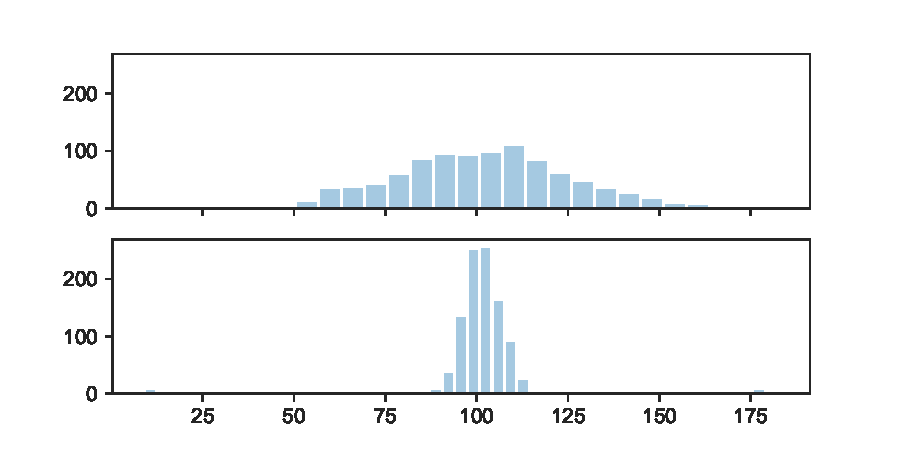
\includegraphics[width=\textwidth]{fig/disp.pdf}

These two datasets both have 1,000 observations \\
that range from about 10 to about 180.
\end{frame}


\begin{frame}{Standard deviation (SD)}
A measure of the amount of variation,\\
in the same unit as the original data

\begin{description}
    \item[Low SD:] values tend to be close to the mean
    \item[High SD:] values can be much lower/higher than mean
\end{description}

\pause
    \begin{columns}[T]
        \column{0.7\textwidth}
            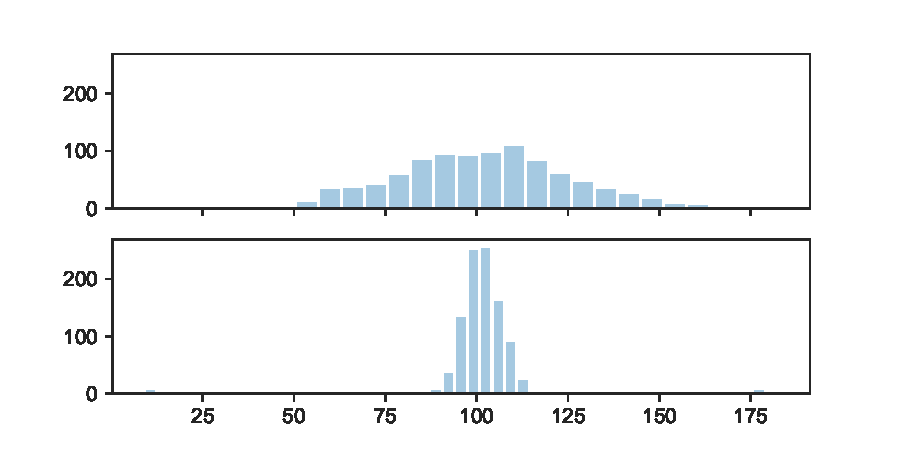
\includegraphics[width=\textwidth]{fig/disp.pdf}
        \column{0.3\textwidth}
            \vspace{3em}
            SD: 24.8

            \vspace{4em}
            SD: 12.9
    \end{columns}
% \begin{block}{Example}
% normal distribution with mean 10 and SD 3, then:\\
% 68\% of values are within 1 SD of mean (between 7 and 13) \\
% 95\% of values are within 2 SDs of mean (between 4 and 16) \\
% 99.7\% \dots
% \dots
% \end{block}
\end{frame}

\begin{frame}{Boxplots (box-and-whisker plot)}
    \begin{reference}
        John W. Tukey (1977). Exploratory Data Analysis. Addison-Wesley.
    \end{reference}
    \begin{columns}[T]
        \column{0.6\textwidth}
            Simple graphical representation of \dots

            \begin{itemize}
                \item Min/max value (whiskers)
                \item Median, 25\% and 75\% quartiles (box)
                \item Optionally: outliers \\
                    (points, excluded from min/max)
            \end{itemize}

        \column{0.4\textwidth}
            Why?
            \begin{itemize}
                \item Useful to show dispersion, skewness, and outliers.

                \item Useful for comparing several distributions.
            \end{itemize}
    \end{columns}

    \pause\centering
    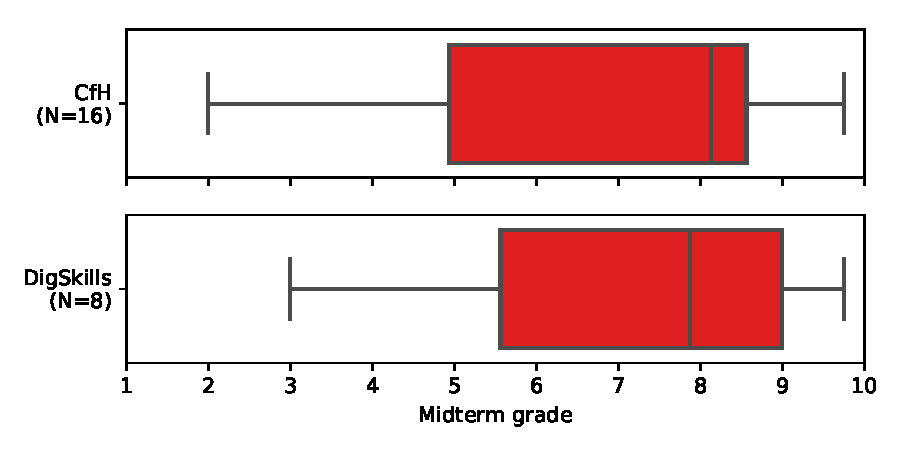
\includegraphics[height=0.5\textheight]{fig/boxplot}
\end{frame}

%\begin{frame}{Boxplot example I: your grades}\centering
%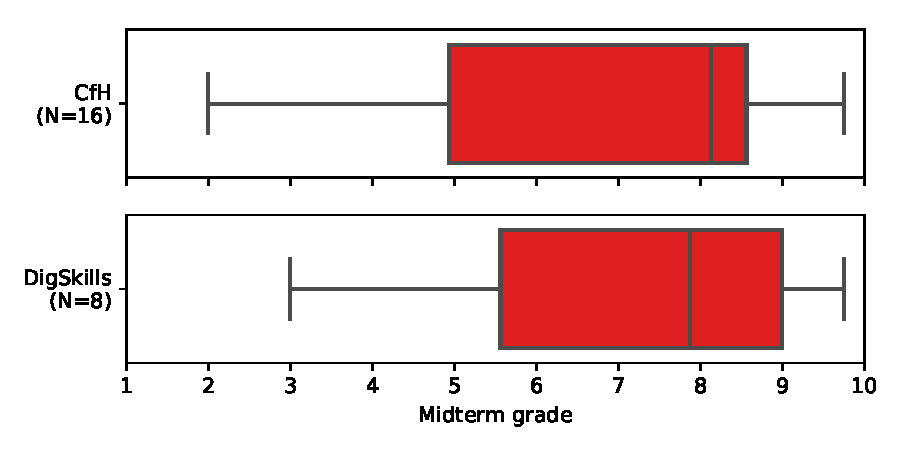
\includegraphics[height=0.8\textheight]{fig/boxplot}
%\end{frame}

\begin{frame}{Boxplot example II}\centering
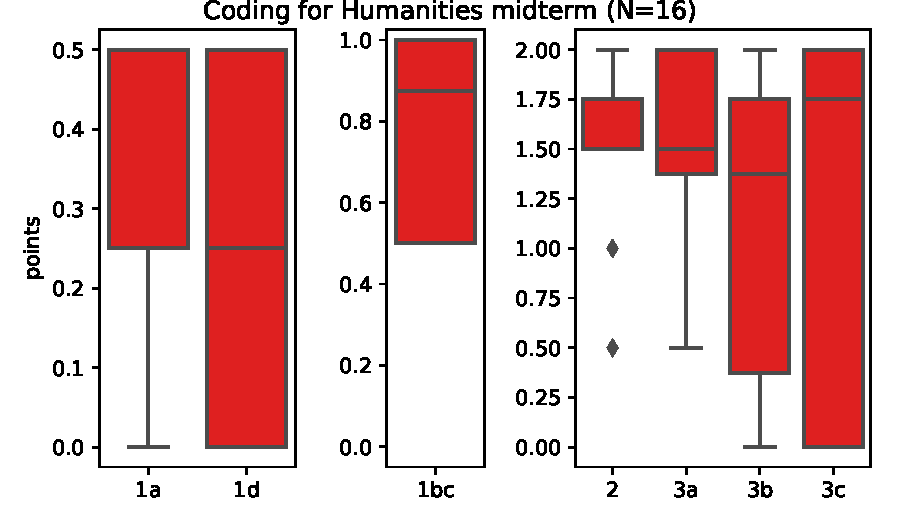
\includegraphics[height=0.75\textheight]{fig/boxplotcmp}

1a counting chars. 1d shorter code. 1bc: better names. \\
2 first letters of poem. 3a find trump tweets. \\
3b count hash tags/usernames. 3c vocabulary richness.
\end{frame}

\begin{frame}{Visualization guidelines (Tufte)}
    \begin{reference}
        Tufte, Edward R (2001/1983), The Visual Display of Quantitative Information.
    \end{reference}
%    \begin{itemize}
%        \item Always provide axis labels
%        \item No misleading scales
%    \end{itemize}
\begin{enumerate}
    \item Represent numbers in a way that is directly proportional to numeric quantities depicted
    \item Use clear and thorough labelling to defeat distortion and ambiguity
    \item Show data variation, not design variation
    \item [\dots]
    % \item If representing money, use deflated and standardized units
    % \item Don't use more information-carrying dimensions than the number of dimensions in the data
    % \item Don't quote data out of context
    % \item Take care of use of absolute values: they may be misleading due to hidden variables
\end{enumerate}
\end{frame}

\begin{frame}{Summary: inspecting one variable}
\noindent\begin{tabular}{@{}lll} & categorical & continuous \\ \midrule
        1. Plot distribution     & bar plot    & histogram, boxplot \\
        2. Central tendency      & mode        & mean, median \\
        3. Dispersion            & -           & range, standard deviation \\
\end{tabular}
\end{frame}




\section{Reproducible research}
\frame{\tableofcontents[currentsubsection]}

\begin{frame}{Intermezzo: reproducibility}
    \structure{Austerity policy}.

    Time line:
    \begin{itemize}
        \item 2008: Economic recession/crisis
        \item Reinhart \& Rogoff (2010) analyze correlation between debt and
            economic growth \\
            \begin{block}{Claim:}
            debt should be less than 90\% of GDP, otherwise economic growth
                drops dramatically
            \end{block}
        \item Austerity policy in EU, Greece needs to reduce debt etc.
    \end{itemize}
\end{frame}

\begin{frame}{The dangers of Excel}
    \begin{reference}
    \url{https://www.nytimes.com/2013/04/19/opinion/krugman-the-excel-depression.html}
    \end{reference}

    Problem:
    \begin{itemize}
        \item The claim is wrong.
            They made a crucial mistake in their Excel sheet!
        \item Excel hides formulas, easy to overlook mistakes
        \item Can we do better with Python?
    \end{itemize}

\end{frame}

\begin{frame}{Reproducibility}
    Research should be reproducible:

    \begin{itemize}
        \item Code and data should be made available \\
            But: \structure{check permissions}! (copyright, licenses)
        \item Code: version control (cf.\ \href{http://www.github.com}{GitHub}),\\
            Data: durable storage in simple formats (text-based)
        \item Make reproducing results \structure{as simple as possible}
        \item Ensure code still works 20+ years later. \\
            Hard problem: ``bit rot''
        \item Audit code/data in peer review \\
            However, this requires lots of time and expertise; realistic?
    \end{itemize}

    %Overlap between open source, open science, open data, open access, etc.
    Can use Jupyter Notebooks for code, results, and documentation. \\
    Only need to store data separately.
\end{frame}


\subsection{Analyzing results with Pandas}
\frame{\tableofcontents[currentsubsection]}

\begin{frame}{Pandas}
    Pandas: versatile data analysis tool \dots

    \begin{itemize}
        \item Load/write tabular data (csv, excel)
        \item Manipulate/process data
        \item Analyze: e.g., basic statistics
        \item Plot: look at data, interactions, etc.
    \end{itemize}
\end{frame}

\begin{frame}{The main datastructures}
    \begin{description}
        \item[Series:] one-dimensional, indexed array of numbers or strings
            \begin{itemize}
                \item ordered (like list)
                \item indexed: lookup items by key (like dict)
                \item mutable
            \end{itemize}
        \item[DataFrame:] two-dimensional table with Series as columns.
            \begin{itemize}
                \item Rows are instances (observations, individuals, etc.)
                \item Columns are features (e.g., age, length, etc.)
            \end{itemize}
            %Each column is a series with a single type (homogeneous), \\
            %but a data frame can contain columns of different types (heterogeneous).
    \end{description}
\end{frame}

% TODO: don't show too much mechanics of Pandas
% show examples, point to further docs, practice during lab in notebook
\begin{frame}[fragile]{Creating a Series}
    \begin{lstlisting}
    In: import pandas as pd
    In: data = pd.Series([0, 1, 2, 3, 4])
    \end{lstlisting}

    \vspace{1em}
    BTW: "as pd" gives a shorter name to the module, \\
    saves a few keystrokes \dots
\end{frame}

\begin{frame}[fragile]{A first plot}
    \begin{lstlisting}
    %matplotlib inline
    data.plot()
    \end{lstlisting}
    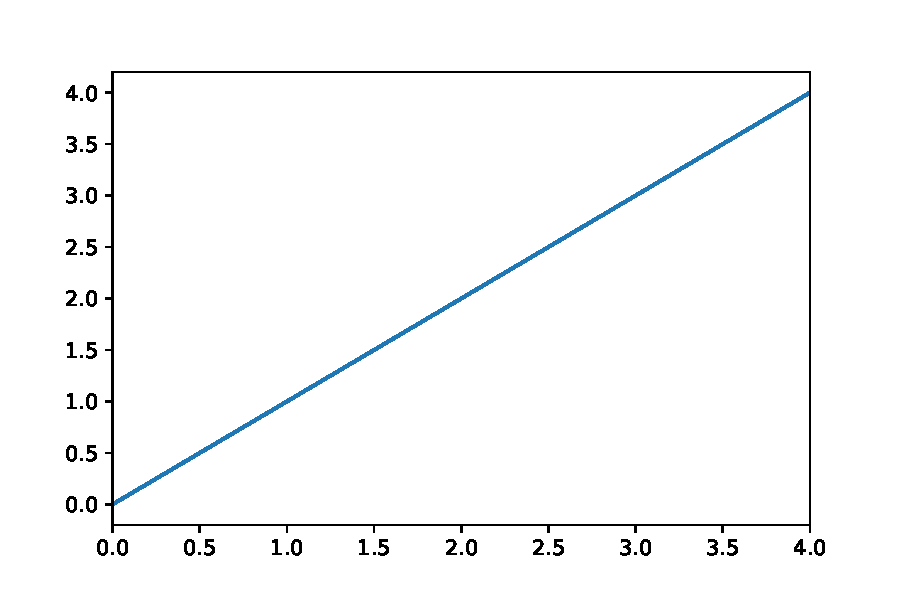
\includegraphics[height=0.5\textheight]{fig/basicplot}
    \pause

Saving the plot (e.g., to include in a report):
\begin{lstlisting}
ax = data.plot()
ax.figure.savefig('plot.pdf')  # PDF
ax.figure.savefig('plot.png', dpi=150)  # PNG
\end{lstlisting}
\end{frame}

\begin{frame}[fragile]{Labeled data}
Two ways:
\begin{lstlisting}
In: data = pd.Series([0, 1], index=['a', 'b'])
In: data = pd.Series({'a': 0, 'b': 1})
Out: Index(['a', 'b'], dtype='object')
\end{lstlisting}

\begin{itemize}
    \item Each datapoint will have a label, \\
        stored in the \texttt{index}.
    \item If no labels are supplied, \\
        a numeric index is automatically created
\end{itemize}
\end{frame}

\begin{frame}[fragile]{Basic statistics}
The sentence lengths of the first night of 1001 Nights:
\begin{columns}
\column{0.5\textwidth}
\begin{lstlisting}
In: lengths = [len(sent) for sent in corpus[0]]
In: data = pd.Series(lengths)
In: data.describe()
Out:
\end{lstlisting}
\begin{lstlisting}[style=plain]
count    378.000000
mean      30.084656
std       17.915458
min        1.000000
25%       17.000000
50%       28.000000
75%       40.750000
max      103.000000
dtype: float64
\end{lstlisting}
\column{0.5\textwidth}
    NB:
    \begin{itemize}
        \item std is the standard deviation.
        \item 50\% is the median.
    \end{itemize}
\end{columns}
\end{frame}


\begin{frame}[fragile]{A boxplot}
The sentence lengths of the first night of 1001 Nights:
\begin{lstlisting}
import seaborn as sns
data = pd.Series(lengths, name='Sentence length')
sns.boxplot(data)
\end{lstlisting}
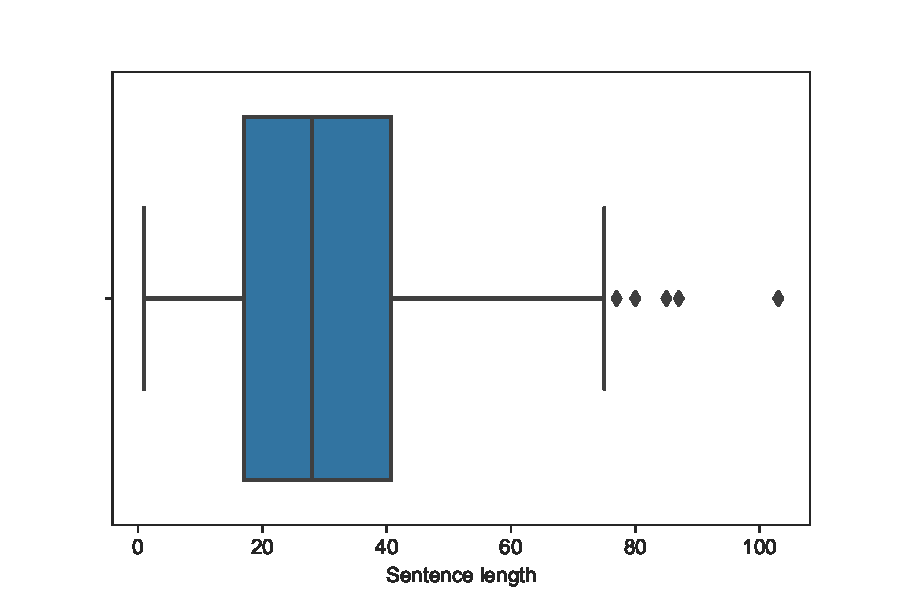
\includegraphics[height=0.65\textheight]{fig/boxplotsents}
\end{frame}

\begin{frame}[fragile]{A histogram}
The sentence lengths of the first night of 1001 Nights:
\begin{lstlisting}
data.hist()
\end{lstlisting}
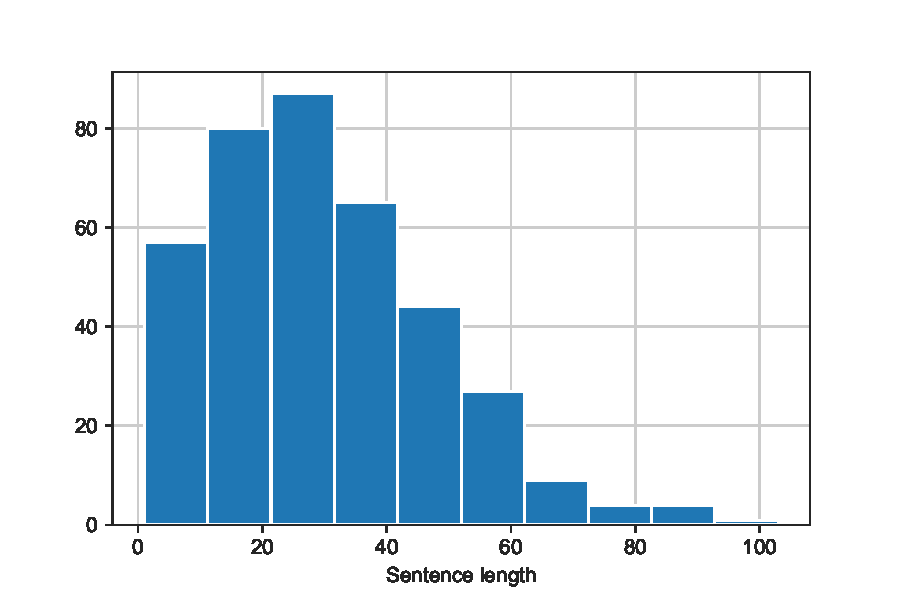
\includegraphics[height=0.7\textheight]{fig/basichist}
\end{frame}


\begin{frame}[fragile]{Counting values: value\_counts()}
\begin{lstlisting}
import nltk
with open('data/arabian_nights/1.txt', encoding='utf8') as infile:
    tokens = nltk.word_tokenize(infile.read())
data = pandas.Series(tokens)
data.value_counts()
\end{lstlisting}
\begin{lstlisting}[style=plain]
and       770
,         730
the       582
of        290
to        286
... 
mer         1
pocket      1
dung        1
Thus        1
farmer      1
Length: 2473, dtype: int64
\end{lstlisting}
\end{frame}

\begin{frame}[fragile]{Counting values: bar plot}
\begin{lstlisting}
counts = data.value_counts()
top20 = counts.head(20)
top20.plot.barh();
\end{lstlisting}
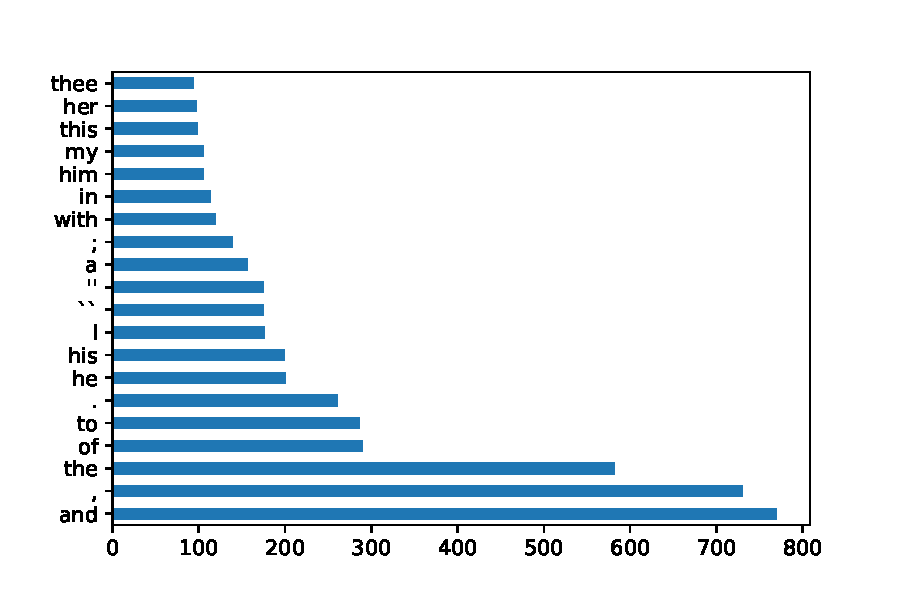
\includegraphics[width=0.7\textwidth]{fig/barplotwords}
\end{frame}

% show more?
% tail
% sort_values, sort_index
% ...

\begin{frame}{Lab}
\begin{itemize}
    \item Finish notebook chapter 3 and week 5 exercises!
    \item Explore \& visualize 1001 nights \& Gutenberg corpus
\end{itemize}
\end{frame}

\begin{frame}
Materials used for these slides:
\begin{itemize}
\item \url{https://www.cs.umd.edu/class/fall2018/cmsc320/}
    specifically lecture 11
    % https://www.cs.umd.edu/class/fall2018/cmsc320/lecs/cmsc320_f2018_lec11.pdf
\end{itemize}

\vspace{1em}
Documentation:
\begin{itemize}
    \item \url{http://pandas.pydata.org/pandas-docs/stable/}
    \item \url{https://seaborn.pydata.org/}
\end{itemize}
\end{frame}

\end{document}
